\documentclass[]{AVSSimReportMemo}
\usepackage{AVS}
\usepackage{colortbl}

\newcommand{\ModuleName}{inertial3D}
\newcommand{\subject}{Guidance Module to Perform an Inertially Fixed Pointing}
\newcommand{\status}{Initial Version}
\newcommand{\preparer}{M. Cols}
\newcommand{\summary}{Generate the reference attitude trajectory for a general 3D inertial pointing.  A corrected body frame will align with the desired reference frame.     }


\begin{document}


\makeCover


%
%	enter the revision documentation here
%	to add more lines, copy the table entry and the \hline, and paste after the current entry.
%
\pagestyle{empty}
{\renewcommand{\arraystretch}{2}
\noindent
\begin{longtable}{|p{0.5in}|p{4.5in}|p{1.14in}|}
\hline
{\bfseries Rev}: & {\bfseries Change Description} & {\bfseries By} \\
\hline
Draft & initial copy & M. Cols \\
\hline

\end{longtable}
}

\newpage
\setcounter{page}{1}
\pagestyle{fancy}

\tableofcontents
~\\ \hrule ~\\

\section{Module Input and Output}
Table \ref{tab:inputTable} shows the input Configuration Data of the module Inertial 3D Point.
\begin{table}[h!]
	\centering
	\caption{Input Configuration Data}
	\begin{tabular}{|l|l|l|p{3in}|}
		\hline
		\rowcolor{BrickRed}
		\textcolor{white}{Name} & \textcolor{white}{Type} & 
		\textcolor{white}{Length} & 
		\textcolor{white}{Description}  \\ \hline
		$\sigma_{R_0/N}$ & double [] & 3 & 
		MRP attitude set of the desired reference frame with respect to the inertial frame . \\ \hline
	\end{tabular}
	\label{tab:inputTable}
\end{table}

Table \ref{tab:outputTable} shows the Attitude Reference output message of the module Inertial 3D Point.
\begin{table}[h!]
	\centering
	\caption{Output Attitude Reference Message}
	\begin{tabular}{|l|l|l|p{3in}|}
		\hline
		\rowcolor{BrickRed}
		\textcolor{white}{Name} & \textcolor{white}{Type} & 
		\textcolor{white}{Length} & 
		\textcolor{white}{Description}  \\ \hline
		$\sigma_{R/N}$ & double [] & 3 & 
		MRP attitude set of the reference frame with respect to the inertial frame. \\ \hline
		$\leftexp{N} \omega_{R/N}$ & double [] & 3 & 
		Angular rate vector of the reference frame with respect to the inertial expressed in inertial frame components. \\ \hline
		$\leftexp{N} {\dot{\omega}_{R/N}}$ & double [] & 3 & 
		Angular acceleration vector of the reference frame with respect to the inertial expressed in inertial frame components. \\ \hline
	\end{tabular}
	\label{tab:outputTable}
\end{table}
\newpage

\section{Introduction}
This technical note discusses the guidance mathematics to compute a reference frame $\mathcal{R}$ that is aligned the with an inertially fixed  frame  $\mathcal{R}_0$, as shown in Figure~\ref{fig:Fig1}.
\begin{figure}[htb]
	\centerline{
	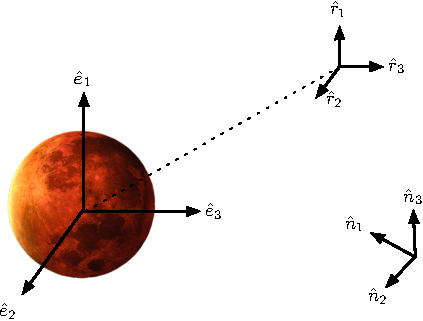
\includegraphics{Figures/Fig3}
	}
	\caption{Illustration of the input inertially fixed frame $\mathcal{R}_{0}:\{ \hat e_{1}, \hat e_{2}, \hat e_{3} \}$, the generated reference frame $\mathcal{R}: \{ \hat r_{1}, \hat r_{2}, \hat r_{3}\}$ and the inertial frame $\mathcal{N}:\{ \hat{\bm n}_{1}, \hat{\bm n}_{2}, \hat{\bm n}_{3} \}$}
	\label{fig:Fig1}
\end{figure}

\section{Reference Frame Generation}
The modules requires the desired reference orientation in terms of the MRP set $\bm{\sigma}_{R_{0}N}$. This input is only set once and does not have to be changed.
Let us designate $\mathcal{R}$ as the output generated reference frame. Since the fixed-pointing is inertial:
\begin{equation}
	\bm{\sigma}_{RN} = \bm{\sigma}_{R_{0}N}
\end{equation}
\begin{equation}
	\bm{\omega}_{RN} = \dot{\bm{\omega}}_{RN} = 0
\end{equation}

\bibliographystyle{unsrt}
\bibliography{references}

\end{document}
